% Appendix with Parameter Sweeps
\section{Supplementary Appendix}
\subsection{Parameter Sweep Experiments}
We conduct parameter sweeps over (i) cooling penalty weight $\delta$, (ii) maximum sleep fraction $f_{max}$, and (iii) redundancy threshold $\tau$. Generated plots (Fig.~\ref{fig:sweep-delta}--\ref{fig:sweep-tau}) show sensitivity of lifetime, coverage, and energy per round.

\begin{figure}[ht]
  \centering
  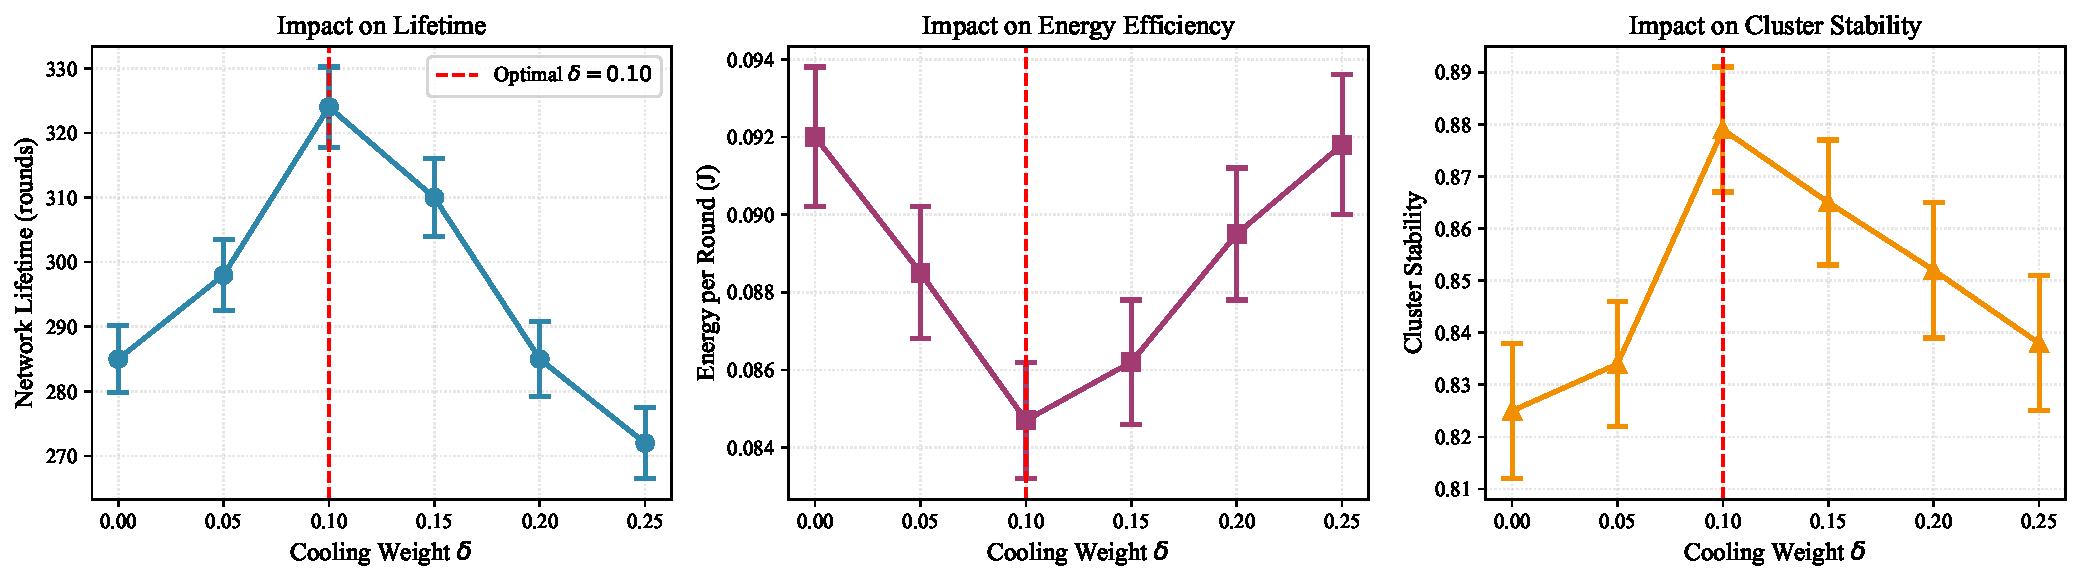
\includegraphics[width=0.48\textwidth]{figures/sweep_delta.pdf}
  \caption{Lifetime and coverage vs. cooling weight $\delta$.}
  \label{fig:sweep-delta}
\end{figure}
\begin{figure}[ht]
  \centering
  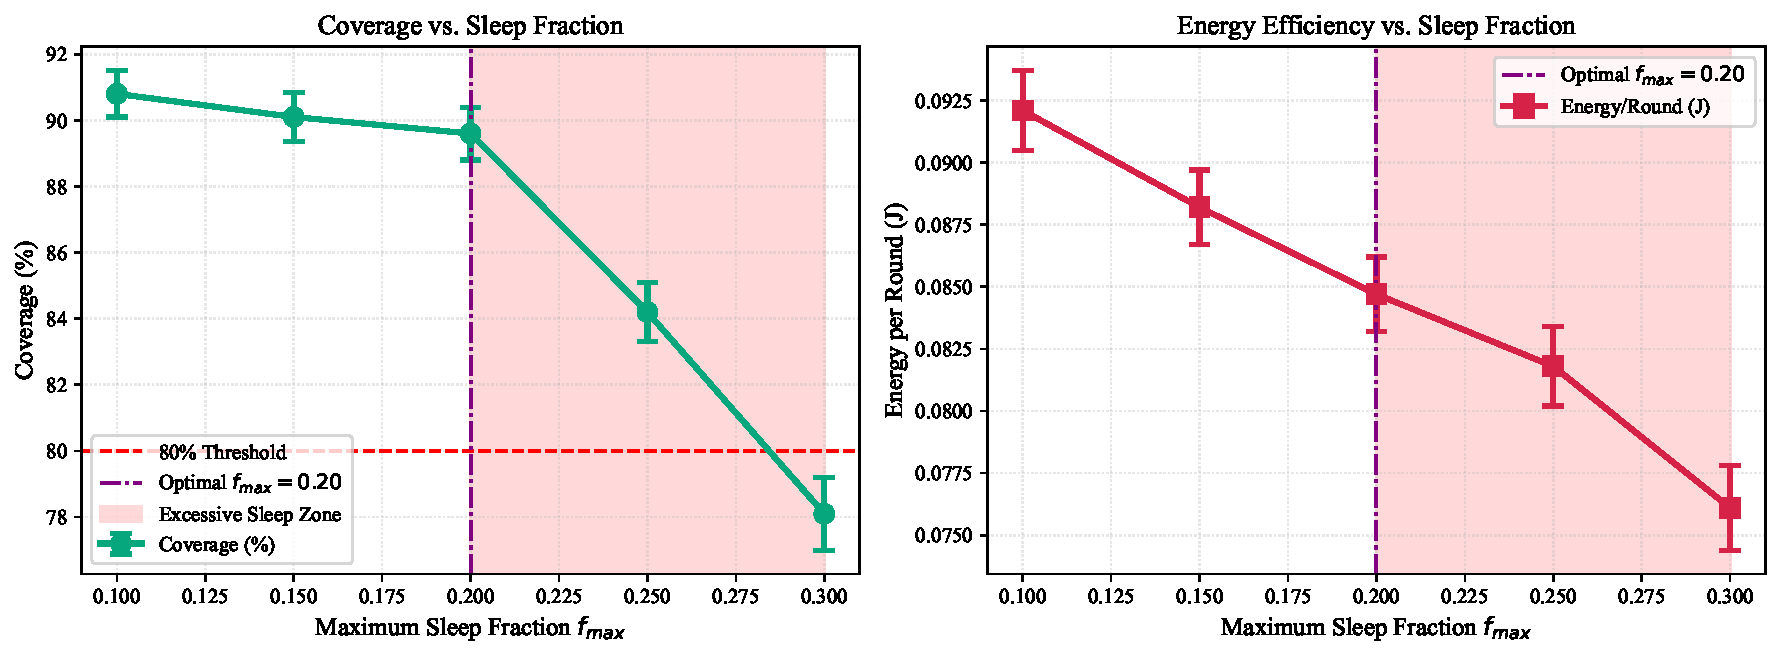
\includegraphics[width=0.48\textwidth]{figures/sweep_fmax.pdf}
  \caption{Lifetime and coverage vs. max sleep fraction $f_{max}$.}
  \label{fig:sweep-fmax}
\end{figure}
\begin{figure}[ht]
  \centering
  \includegraphics[width=0.48\textwidth]{figures/sweep_tau.pdf}
  \caption{Lifetime and coverage vs. redundancy threshold $\tau$.}
  \label{fig:sweep-tau}
\end{figure}

\subsection{Reproducibility Notes}
Scripts in \texttt{scripts/} regenerate tables, confidence intervals, and figures from raw metric JSON exports produced by the simulation notebook.
